%  http://latex-beamer.sourceforge.net/

%\documentclass[landscape]{foils}

%\documentclass{beamer}
%\documentclass[handout]{beamer}     % TO PRINT PRESENTATION HANDOUT
\documentclass[xcolor=dvipsnames]{beamer}  % ALLOWS CHANGE IN COLOR

\usepackage{color}

\usepackage{pifont} %para tener la ballot cross \ding{55}

\usepackage{beamerthemesplit}
\usepackage{url}
\usepackage{ae} % or {zefonts}
\usepackage[T1]{fontenc}
\usepackage[ansinew]{inputenc}
\usepackage[spanish]{babel}

\usepackage{graphicx}
%\graphicspath{"c:/data"}
\usepackage{color}
\usepackage{hyperref}
\usepackage{tikz} % Easier syntax to draw pgf files (invokes pgf automatically)
\usetikzlibrary{arrows,shapes.geometric}
%\usepackage{pgfmath}


%\usecolortheme{crane}     %Color yellow
%\usetheme{Warsaw}
\usecolortheme[named=Gray]{structure}

\useoutertheme[footline=empty]{}  % PUTS COLORED LINE AT FOOT WITH TITLE, AUTHOR, PAGE, etc
%\usetheme{Berkeley}
\usetheme[height=7mm]{Rochester}
\setbeamertemplate{items}[ball]   % ITEMS IN 3D BALLS (alt CIRCLES)
\setbeamertemplate{navigation symbols}{}  % DROPS NAVIGATION ICONS
\setbeamertemplate{blocks}[rounded][shadow=true]

\usepackage{multirow} %allows multiple rows in tables

%\setbeamertemplate{footline} {
%    \begin{beamercolorbox}{section in head/foot}
%    \insertsectionnavigationhorizontal{\paperwidth}{}{plus1filll
%    \insertframenumber}
%    \end{beamercolorbox}
%}


%\setbeamertemplate{navigation symbols}{\insertslidenavigationsymbol,
%\insertdocnavigationsymbol} \setbeamertemplate{footline} {
%    \begin{beamercolorbox}{section in head/foot}
%    \insertsectionnavigationhorizontal{\paperwidth}{}{plus1filll
%    \insertframenumber}
%    \end{beamercolorbox}
%}

\setbeamercovered{transparent}
\setbeamertemplate{caption}{\insertcaption}

% \AtBeginSection[] {
%    \begin{frame}
%        \frametitle{Outline}
%        \tableofcontents[currentsection]
%    \end{frame}
% }

\tikzstyle{nodo} = [circle, draw=black, fill=white, text=black]
\tikzstyle{end} = [circle, minimum width=3pt,fill, inner sep=0pt]

\usepackage{array,tabto} % allows word jumps to specific distance \tabto{2cm}

% read external link symbol code store in current directory
% usage: \ExternalLink
%%%%%%%%%%%%%%%%%%%%%%%%%%%%%%%%%%%%%%%%%%%%%%%%%%%%%%%%%%%%%%%%%%%%%%%%%%%%%%%%%%%%%%%%
%% TEX code to draw an external link symbol                                           %%
%% See https://tex.stackexchange.com/questions/99316/symbol-for-external-links/294990 %%
%%%%%%%%%%%%%%%%%%%%%%%%%%%%%%%%%%%%%%%%%%%%%%%%%%%%%%%%%%%%%%%%%%%%%%%%%%%%%%%%%%%%%%%%

\usepackage{tikz}

\newcommand{\ExternalLink}{%
    \tikz[x=1.2ex, y=1.2ex, baseline=-0.05ex]{% 
        \begin{scope}[x=1ex, y=1ex]
            \clip (-0.1,-0.1) 
                --++ (-0, 1.2) 
                --++ (0.6, 0) 
                --++ (0, -0.6) 
                --++ (0.6, 0) 
                --++ (0, -1);
            \path[draw, 
                line width = 0.5, 
                rounded corners=0.5] 
                (0,0) rectangle (1,1);
        \end{scope}
        \path[draw, line width = 0.5] (0.5, 0.5) 
            -- (1, 1);
        \path[draw, line width = 0.5] (0.6, 1) 
            -- (1, 1) -- (1, 0.6);
    }
}




\title[Slippage at IFE]{Slippage among the Experts}
\subtitle{Agency Costs in Partisan Election Regulation}
\author[Est\'evez, Magar \& Rosas]{Federico Est\'evez\inst{1} \and Eric Magar\inst{1} \and Guillermo Rosas\inst{2}}
\institute[ITAM\&WashU]{ \inst{1}ITAM, Mexico City \and
\inst{2}Wash.~U., St.~Louis}
\date[6/25/22]{6/25/22 \\ \small{Mat McCubbins Memorial Conference, UCSD} }

\begin{document}

%%%%%%%%%%%%%%%%%%%%%%%%%%%%%%%%%%%%%%%%%%%%%%%%%%%%%%%%%%%%%%%%%%%%%%%%%%%%%%%%%%%%%%%%%%%%%%%%

\frame[plain]{\titlepage}

%%%%%%%%%%%%%%%%%%%%%%%%%%%%%%%%%%%%%%%%%%%%%%%%%%%%%%%%%%%%%%%%%%%%%%%%%%%%%%%%%%%%%%%%%%%%%%%%
\frame {                      % SLIDE

%    \frametitle{Our work on IFE, now and then}
    \frametitle{Our work on Mexican election regulation}

%How does delegation work in fast-changing, multi-party systems?

%\bigskip

\begin{description}

\item[Before:] Party watchdog model, congressional parties delegate %\\
% {\footnotesize (Est�vez, Magar, Rosas 2008)}

\begin{itemize}
\item Expect party segmentation of IFE's Council General
\item Ideal point estimation confirms
\end{itemize}

\bigskip

\item[Now:] Longitudinal approach to study councilor drift 1996--2014

\begin{itemize}
\item Still exploratory
\item New puzzles emerge 
\end{itemize}

\end{description}

% \pause \pause \bigskip

% $\rightarrow$ Key pieces of the structure of delegation missing in Mexico:

% \begin{enumerate}
% \item Multi- vs. two-party system %, some compromise to pass senate, majority can set long-term policy
% \item Constant mutation vs. stability
% \item Younger vs. mature bureaucrats
% \end{enumerate}

}
%%%%%%%%%%%%%%%%%%%%%%%%%%%%%%%%%%%%%%%%%%%%%%%%%%%%%%%%%%%%%%%%%%%%%%%%%%%%%%%%%%%%%%%%%%%%%%%%
% %\section{Outline}

% \frame {                      % SLIDE

%     \frametitle{Outline}

% \tableofcontents[section=1]

% }
%%%%%%%%%%%%%%%%%%%%%%%%%%%%%%%%%%%%%%%%%%%%%%%%%%%%%%%%%%%%%%%%%%%%%%%%%%%%%%%%%%%%%%%%%%%%%%%%
%\section{IFE and delegation}
\frame {                      % SLIDE

    \frametitle{The Federal Electoral Institute (IFE)}

\begin{itemize}

\item Nine-member, non-partisan regulatory board
\item Ran federal elections nationwide 1997--2012
% \item Congress appoints members (super-majority) for 7-year terms. Party quota/veto system (informal)
\item Congress appoints members by super-majority for 7-year terms
\item Public roll call votes
\item Upgraded in 2014 to also regulate subnational races (INE)
  
\end{itemize}

\bigskip \bigskip \pause \centering PRI (later others) conceded, \\\textbf<2>{how did IFE achieve this?}

}
%%%%%%%%%%%%%%%%%%%%%%%%%%%%%%%%%%%%%%%%%%%%%%%%%%%%%%%%%%%%%%%%%%%%%%%%%%%%%%%%%%%%%%%%%%%%%%%%
\frame {                      % SLIDE

    \frametitle{IFE's success story: conventional arguments}

\begin{itemize}
\item IFE as \emph{ombusdman} representing citizens directly \\ {\color{black!25} \footnotesize (Eisenstadt 2004, Ackerman 2004)}
\item Budget and tenure security
\item Congressional appointment yet no inevitable bias in experts {\color{black!25} \footnotesize (Schedler 2000, Woldenberg 2008)}
\end{itemize}

\bigskip

\begin{center}
Independence + impartiality $\rightarrow$ citizen trust
\end{center}

\pause \bigskip

\begin{block}{Public opinion}
\centering
{\footnotesize 
  \begin{tabular}{lr}
                & \% trust  \\ \hline
    Church      & 72 \\
    \textbf{IFE} & \textbf{67} \\
    Army        & 65 \\
    Congress    & 35 \\
    Parties     & 34 \\ \hline
    \multicolumn{2}{r}{\tiny \emph{Reforma} poll May 2005}\\
  \end{tabular} 
}
\end{block}
}
%%%%%%%%%%%%%%%%%%%%%%%%%%%%%%%%%%%%%%%%%%%%%%%%%%%%%%%%%%%%%%%%%%%%%%%%%%%%%%%%%%%%%%%%%%%%%%%%
\frame {                      % SLIDE

    \frametitle{Our argument owes much to Mat}

% {\footnotesize     
%   \onslide<2-> \tabto{.8cm}\textbf{parties} \tabto{8.05cm}\textbf{IFE}\\
%                \tabto{1.15cm}$\updownarrow$ \tabto{8.2cm}$\updownarrow$ \\
% \onslide<1-> ``The \alert<2->{principal} seeks to structure the relationship with the \alert<2->{agent} so that the outcomes produced through the agent's efforts are the best the principal could achieve, given the choice to delegate in the first place'' \\ (Kiewiet \& McCubbins 1991:24)
% }
    
Congressional parties (principal) structure a referee (agent) that they can influence %\\  (Kiewiet \& McCubbins 1991, McNollgast 1987)

% \bigskip

% scope + instruments $-$ procedures = agency discretion\\
% (+) (+) (++) (--) $\leftarrow$ uncertainty/conflict \\
% {\footnotesize(McCubbins and Page 1986)}

\pause \bigskip

High stakes: IFE has authority over every aspect of party life

\begin{itemize}
\begin{columns}
\column{.3\textwidth}
        \item voter registration
        \item redistricting
        \item nominations
        \item campaign content
\column{.4\textwidth}
        \item allocates TV spots
        \item campaign finance
%        \item leaders v.\ rank-and-file
        \item who clears subsidy hurdle
        \item ...
\end{columns}
\end{itemize}

\pause \bigskip

\centering
Careful delegation $\rightarrow$ \textbf{party} trust $\rightarrow$ citizen trust
}
%%%%%%%%%%%%%%%%%%%%%%%%%%%%%%%%%%%%%%%%%%%%%%%%%%%%%%%%%%%%%%%%%%%%%%%%%%%%%%%%%%%%%%%%%%%%%%%%
\frame {                      % SLIDE

    \frametitle{Our argument}
\begin{block}{Contract design (Kiewiet \& McCubbins 1991)}
 \begin{center}
    \begin{itemize}
    \item<1-> Screening
      \begin{itemize}
      \item<2> formally non-partisan
      \item<2> super-majority rule
      \item<2> party quotas/veto (informal)
      \end{itemize}
    \item<1-> Monitoring
      \begin{itemize}
      \item<3> party reps in board and committees
      \item<3> constant signalling
      \end{itemize}
    \item<1-> Carrots/sticks
      \begin{itemize}
      \item<4> routine impeachment threats, some took place
      \item<4> budget cuts
      \item<4> nuclear option (electoral reform)
      \end{itemize}
    \item<1-> Checks and balances
      \begin{itemize}
      \item<5> split in thirds
      \item<5> electoral tribunal
      \end{itemize}
    \end{itemize}
 \end{center}
\end{block}
}
%%%%%%%%%%%%%%%%%%%%%%%%%%%%%%%%%%%%%%%%%%%%%%%%%%%%%%%%%%%%%%%%%%%%%%%%%%%%%%%%%%%%%%%%%%%%%%%%
\frame {                      % SLIDE

    \centering 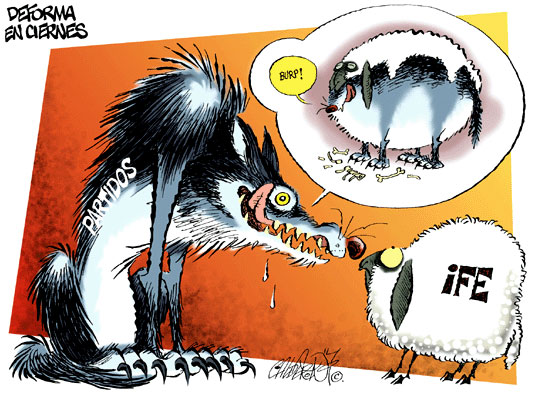
\includegraphics[width=.85\textwidth]{../../pics/calderonIFE20070829.jpg}
    \\ {\color{black!25}\tiny{From \url{http://reforma.com.mx} 8/29/2007}}

}
%%%%%%%%%%%%%%%%%%%%%%%%%%%%%%%%%%%%%%%%%%%%%%%%%%%%%%%%%%%%%%%%%%%%%%%%%%%%%%%%%%%%%%%%%%%%%%%%
%\section{Data and methods}

% \frame {                      % SLIDE

%     \frametitle{Stochastic spatial voting}

% \begin{center}
%  \begin{tikzpicture}[scale=1,rotate=0]
%   \def\xo{0,0}
%   \def\xu{4,0}
%   \def\xj{2.7,0}
%   \def\m{2,0}
%   \draw (-1,0) -- (5,0);
%   \fill[red] (\xo) circle (1.5pt) node [below=2pt,black] {$nay$};
%   \fill[green] (\xu) circle (1.5pt) node [below=2pt,black] {$aye$};
% %  \fill[black] (\xj) circle (1.5pt) node [below=2pt,black] {$x_j$};
%   \draw (2,.1) -- (2,-.1) node [below=2pt,black] {$m$};
% %  \fill[black!50] (\xj) circle (1.5pt) node [below=2pt,black] {$j$};
%  \end{tikzpicture}
% \end{center}

% \bigskip

% {\color{black!15}

% Vote propensity: $y^*_{j}= \delta(x_j - m) +\text{error}$.

% \bigskip

% Voting is sincere: $y_j=
%  \begin{cases}
%   1 \text{ (`aye')} \iff y^*_{j} \geq 0 \\
%   0 \text{ (`nay') otherwise.}           \,
%  \end{cases}$

% \bigskip

% Dynamics: $x_{j,t} \sim \mathrm{N}( x_{j,t-1},\text{slack}
% )$~~~~~(cf.\ Martin\&Quinn 2002).

% \bigskip

% Small assembly: Bayesian estimation via MCMC simulation. }

% }
%%%%%%%%%%%%%%%%%%%%%%%%%%%%%%%%%%%%%%%%%%%%%%%%%%%%%%%%%%%%%%%%%%%%%%%%%%%%%%%%%%%%%%%%%%%%%%%%
\frame {
    \frametitle{Stochastic spatial voting}\label{analogy}
\begin{center}
 \begin{tikzpicture}[scale=1,rotate=0]
  \def\xo{0,0}
  \def\xu{4,0}
  \def\xj{2.7,0}
  \def\m{2,0}
  \draw (-1,0) -- (5,0);
  \fill[red] (\xo) circle (1.5pt) node [below=2pt,black] {$nay$};
  \fill[green] (\xu) circle (1.5pt) node [below=2pt,black] {$aye$};
  \fill[black] (\xj) circle (1.5pt) node [below=2pt,black] {$x_j$};
  \draw (2,.1) -- (2,-.1) node [below=2pt,black] {$m$};
%  \fill[black!50] (\xj) circle (1.5pt) node [below=2pt,black] {$j$};
 \end{tikzpicture}
\end{center}

\bigskip 

Vote propensity: $v^*_{j}= \texttt{signal}(x_j - m) +\texttt{error}$

\bigskip 

Voting is sincere: $v_j=
 \begin{cases}
  1 \text{ (`aye')} \iff v^*_{j} \geq 0 \\
  0 \text{ (`nay') otherwise}           \,
 \end{cases}$

\bigskip

Dynamics: $x_{j,t} \sim \mathrm{N}( x_{j,t-1},\text{slack}
)$ \tabto{6cm} (cf.\ Martin\&Quinn 2002,\\ \tabto{6.2cm} also Bonica 2010 \hyperlink{dyn-slide}{\ExternalLink})

\bigskip 

Small committee: Bayesian estimation via MCMC simulation

\bigskip

\begin{flushright}
{\footnotesize \color{black!25} Identification \hyperlink{identification}{\ExternalLink}}
{\footnotesize \color{black!25} Votes \hyperlink{data}{\ExternalLink}}
\end{flushright}
}
%%%%%%%%%%%%%%%%%%%%%%%%%%%%%%%%%%%%%%%%%%%%%%%%%%%%%%%%%%%%%%%%%%%%%%%%%%%%%%%%%%%%%%%%%%%%%%%%
\frame {
  \frametitle{Expectations}
  Ideal point summarizes member's voting record vis-�-vis rest, \\
  proximity = \alert{vote likeness}
  \bigskip
  % General
  \begin{enumerate}
  \item Contiguity/superimposition of same-sponsor members
  \item Party segmentation
%  Drift
  \item Move in tandem
  \item Gatekeeping: blocking divisive issues brings most together
  \item Vanishing principal: drift should \emph{follow}
%  \item Vote trading: moderates across the fence
  \end{enumerate}
}
%%%%%%%%%%%%%%%%%%%%%%%%%%%%%%%%%%%%%%%%%%%%%%%%%%%%%%%%%%%%%%%%%%%%%%%%%%%%%%%%%%%%%%%%%%%%%%%%
\frame {
  \frametitle{Evidence}
\begin{center}
  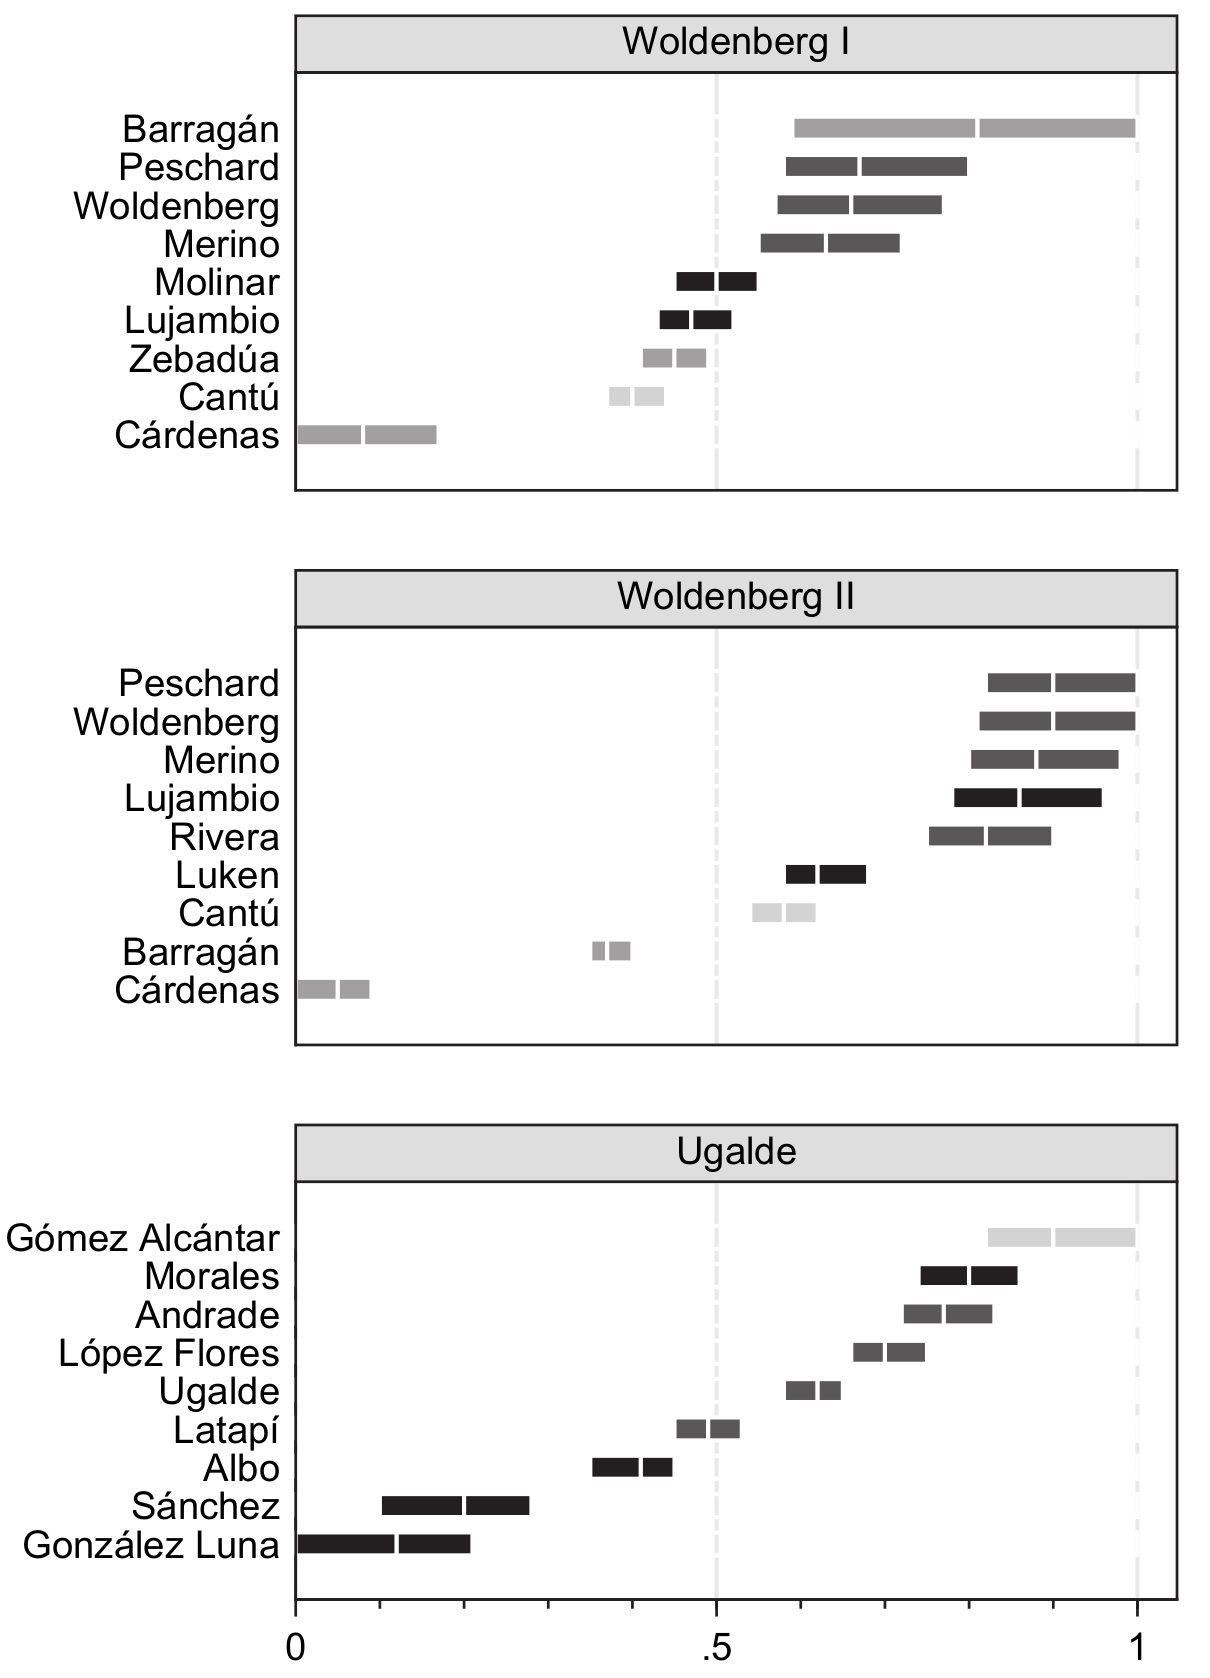
\includegraphics[width=.6\textheight]{../../pics/paper-ips.png} \\
\end{center}
}
%%%%%%%%%%%%%%%%%%%%%%%%%%%%%%%%%%%%%%%%%%%%%%%%%%%%%%%%%%%%%%%%%%%%%%%%%%%%%%%%%%%%%%%%%%%%%%%%
\frame {
  \frametitle{Overview stability \& change}
\begin{center}
 \includegraphics[width=.75\textwidth]{../../../original/graphs/1dimDynWold9703jmayorPrecision.pdf} \\
\end{center}
}
%%%%%%%%%%%%%%%%%%%%%%%%%%%%%%%%%%%%%%%%%%%%%%%%%%%%%%%%%%%%%%%%%%%%%%%%%%%%%%%%%%%%%%%%%%%%%%%%
\frame {
  \frametitle{Overview stability \& change}
\begin{center}
% \includegraphics[width=.75\textwidth]{../../../original/graphs/1dimDynUgalde0307jmayorPrecision.pdf} \\
 \includegraphics[width=.75\textwidth]{../../../original/graphs/1dimDynUgaVal0410j.pdf} \\
\end{center}
}
%%%%%%%%%%%%%%%%%%%%%%%%%%%%%%%%%%%%%%%%%%%%%%%%%%%%%%%%%%%%%%%%%%%%%%%%%%%%%%%%%%%%%%%%%%%%%%%%
\frame {
  \frametitle{Overview stability \& change}
\begin{center}
 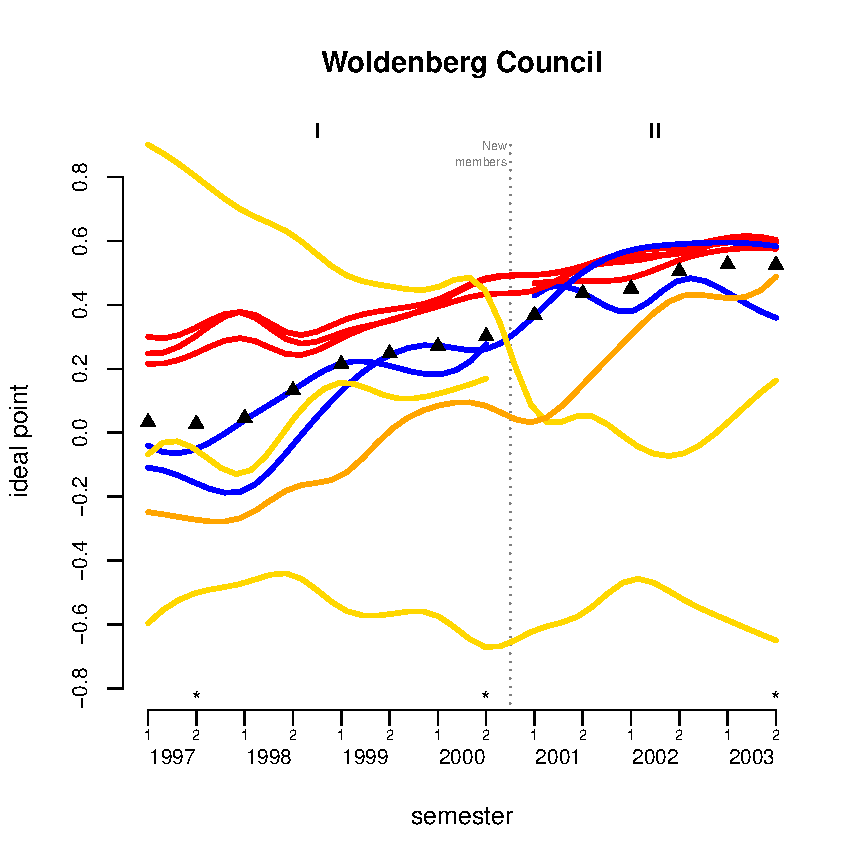
\includegraphics[width=.75\textwidth]{../../../original/graphs/allWdynNoNames.pdf} \\
\end{center}
}
%%%%%%%%%%%%%%%%%%%%%%%%%%%%%%%%%%%%%%%%%%%%%%%%%%%%%%%%%%%%%%%%%%%%%%%%%%%%%%%%%%%%%%%%%%%%%%%%
\frame {
  \frametitle{Overview stability \& change}
\begin{center}
 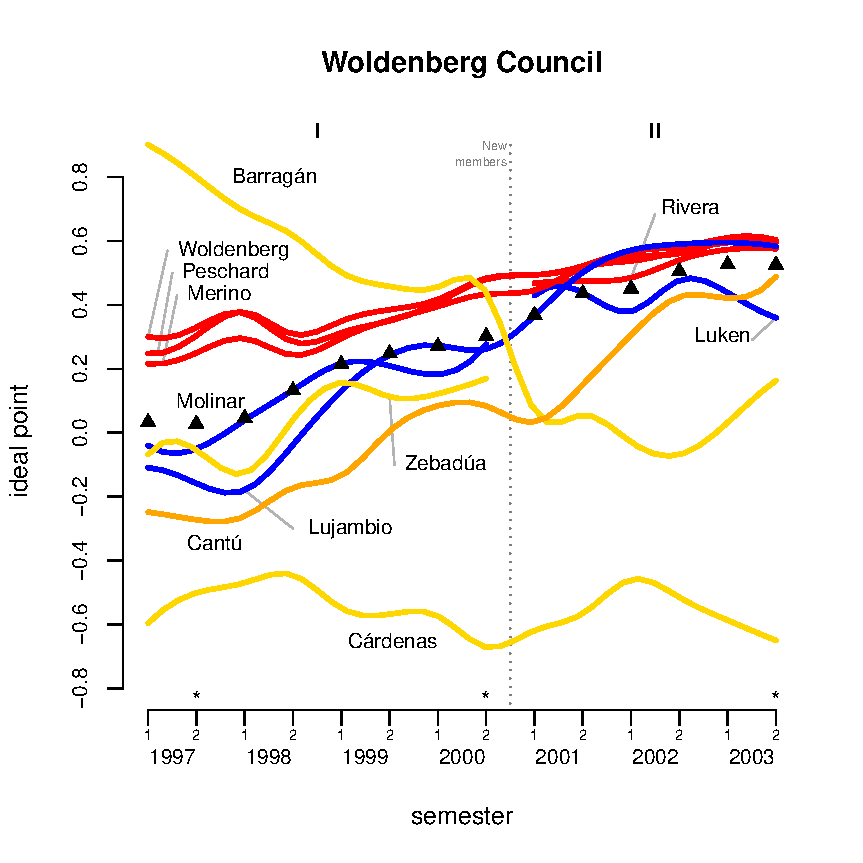
\includegraphics[width=.75\textwidth]{../../../original/graphs/allWdyn.pdf} \\
\end{center}
}
%%%%%%%%%%%%%%%%%%%%%%%%%%%%%%%%%%%%%%%%%%%%%%%%%%%%%%%%%%%%%%%%%%%%%%%%%%%%%%%%%%%%%%%%%%%%%%%%
\frame {
  \frametitle{Overview stability \& change}
\begin{center}
 \includegraphics[width=.75\textwidth]{../../../original/graphs/allUpreV1dynNoNames.pdf} \\
\end{center}
}
% %%%%%%%%%%%%%%%%%%%%%%%%%%%%%%%%%%%%%%%%%%%%%%%%%%%%%%%%%%%%%%%%%%%%%%%%%%%%%%%%%%%%%%%%%%%%%%%%
% \frame {
%   \frametitle{Overview stability \& change}
% \begin{center}
%  \includegraphics[width=.75\textwidth]{../../../original/graphs/allUpreV1dyn.pdf} \\
% \end{center}
% }
%%%%%%%%%%%%%%%%%%%%%%%%%%%%%%%%%%%%%%%%%%%%%%%%%%%%%%%%%%%%%%%%%%%%%%%%%%%%%%%%%%%%%%%%%%%%%%%%
\frame {
  \frametitle{Overview stability \& change}
\begin{center}
 \includegraphics[width=.75\textwidth]{../../../original/graphs/allUVdyn04-10NoNames.pdf} \\
\end{center}
}
%%%%%%%%%%%%%%%%%%%%%%%%%%%%%%%%%%%%%%%%%%%%%%%%%%%%%%%%%%%%%%%%%%%%%%%%%%%%%%%%%%%%%%%%%%%%%%%%
\frame {
  \frametitle{Overview stability \& change}
\begin{center}
 \includegraphics[width=.75\textwidth]{../../../original/graphs/allUVdyn04-10.pdf} \\
\end{center}
}
%%%%%%%%%%%%%%%%%%%%%%%%%%%%%%%%%%%%%%%%%%%%%%%%%%%%%%%%%%%%%%%%%%%%%%%%%%%%%%%%%%%%%%%%%%%%%%%%
\frame {
  \frametitle{Overview stability \& change}
\begin{center}
 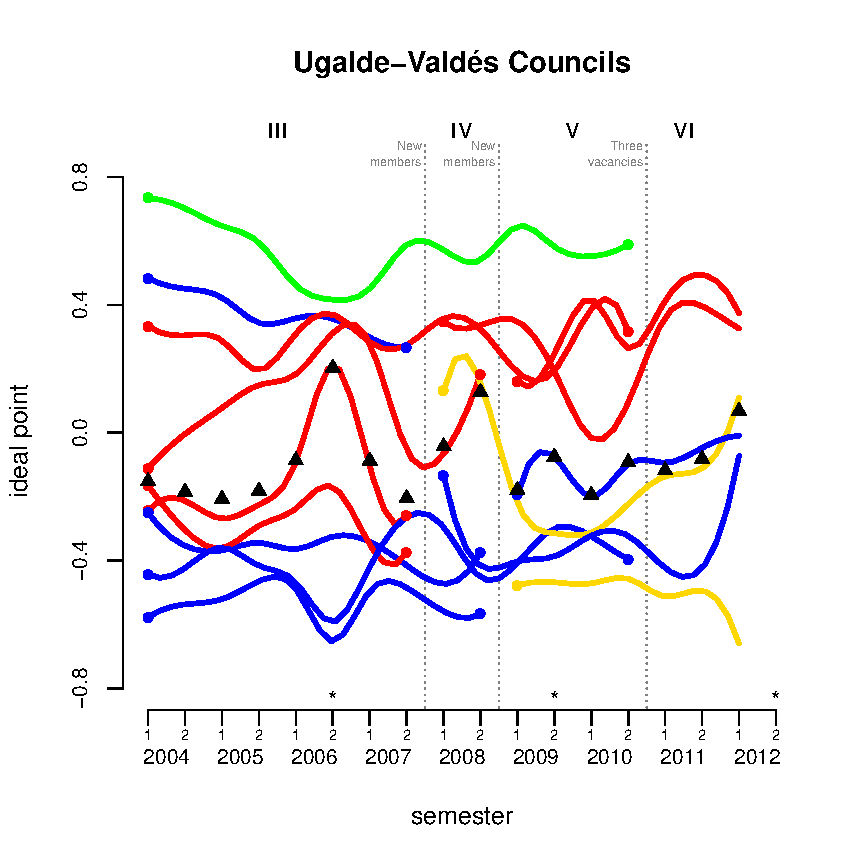
\includegraphics[width=.75\textwidth]{../../../original/graphs/allUVdyn04-12noNames.pdf} \\
\end{center}
}
% %%%%%%%%%%%%%%%%%%%%%%%%%%%%%%%%%%%%%%%%%%%%%%%%%%%%%%%%%%%%%%%%%%%%%%%%%%%%%%%%%%%%%%%%%%%%%%%%
% \frame {
%   \frametitle{Overview stability \& change}
% \begin{center}
%  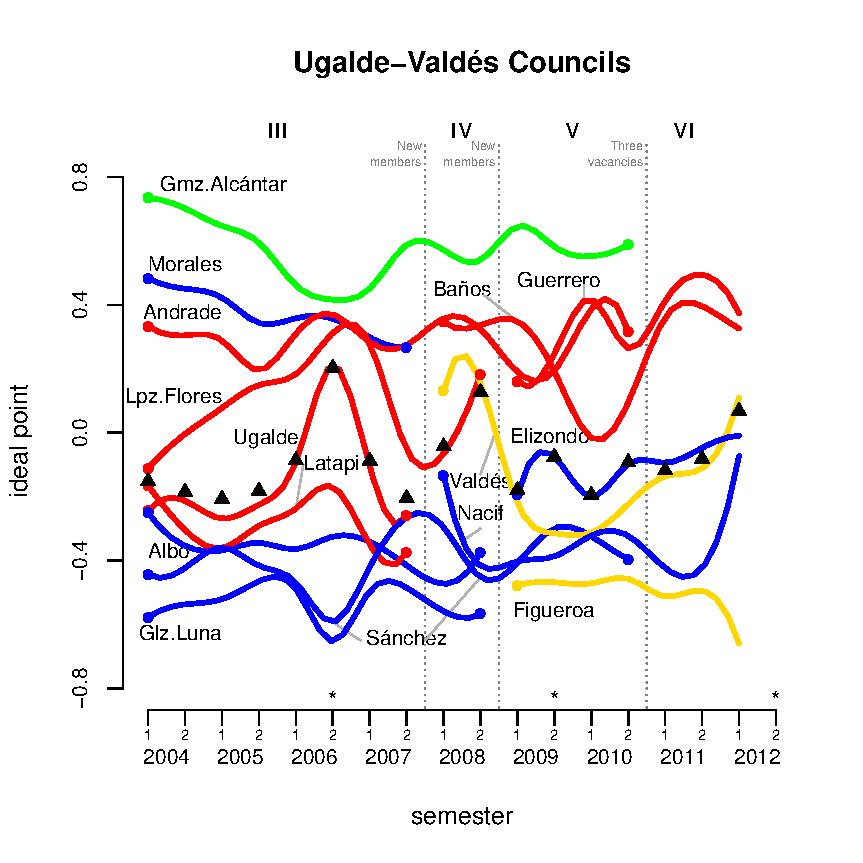
\includegraphics[width=.75\textwidth]{../../../original/graphs/allUVdyn04-12.pdf} \\
% \end{center}
% }
%%%%%%%%%%%%%%%%%%%%%%%%%%%%%%%%%%%%%%%%%%%%%%%%%%%%%%%%%%%%%%%%%%%%%%%%%%%%%%%%%%%%%%%%%%%%%%%%
\frame {
  \frametitle{Clustering and overlaps}
\begin{center}
 \includegraphics[width=.75\textwidth]{../../../original/graphs/woStackPAN.pdf} \\
\end{center}
}
%%%%%%%%%%%%%%%%%%%%%%%%%%%%%%%%%%%%%%%%%%%%%%%%%%%%%%%%%%%%%%%%%%%%%%%%%%%%%%%%%%%%%%%%%%%%%%%%
\frame {
  \frametitle{Clustering and overlaps}
\begin{center}
 \includegraphics[width=.75\textwidth]{../../../original/graphs/woStackPRI.pdf} \\
\end{center}
}
%%%%%%%%%%%%%%%%%%%%%%%%%%%%%%%%%%%%%%%%%%%%%%%%%%%%%%%%%%%%%%%%%%%%%%%%%%%%%%%%%%%%%%%%%%%%%%%%
\frame {
  \frametitle{Clustering and overlaps}
\begin{center}
 \includegraphics[width=.75\textwidth]{../../../original/graphs/woStackPRD.pdf} \\
\end{center}
}
%%%%%%%%%%%%%%%%%%%%%%%%%%%%%%%%%%%%%%%%%%%%%%%%%%%%%%%%%%%%%%%%%%%%%%%%%%%%%%%%%%%%%%%%%%%%%%%%
\frame {
  \frametitle{Clustering and overlaps}
\begin{center}
 \includegraphics[width=.75\textwidth]{../../../original/graphs/UgPRIdyn.pdf} \\
\end{center}
}
%%%%%%%%%%%%%%%%%%%%%%%%%%%%%%%%%%%%%%%%%%%%%%%%%%%%%%%%%%%%%%%%%%%%%%%%%%%%%%%%%%%%%%%%%%%%%%%%
\frame {
  \frametitle{Clustering and overlaps}
\begin{center}
 \includegraphics[width=.75\textwidth]{../../../original/graphs/ugvalStackPAN.pdf} \\
\end{center}
}
%%%%%%%%%%%%%%%%%%%%%%%%%%%%%%%%%%%%%%%%%%%%%%%%%%%%%%%%%%%%%%%%%%%%%%%%%%%%%%%%%%%%%%%%%%%%%%%%
\frame {
  \frametitle{Clustering and overlaps}
\begin{center}
 \includegraphics[width=.75\textwidth]{../../../original/graphs/ugvalStackPRIelba.pdf} \\
\end{center}
}
%%%%%%%%%%%%%%%%%%%%%%%%%%%%%%%%%%%%%%%%%%%%%%%%%%%%%%%%%%%%%%%%%%%%%%%%%%%%%%%%%%%%%%%%%%%%%%%%
\frame {
  \frametitle{Clustering and overlaps}
\begin{center}
 \includegraphics[width=.75\textwidth]{../../../original/graphs/ugvalStackPRImadPVEM.pdf} \\
\end{center}
}
%%%%%%%%%%%%%%%%%%%%%%%%%%%%%%%%%%%%%%%%%%%%%%%%%%%%%%%%%%%%%%%%%%%%%%%%%%%%%%%%%%%%%%%%%%%%%%%% 
\frame {
    \frametitle{Possible empirical indicators}
 \begin{itemize}
  \item New Congress (also party splits) $\rightarrow$ principals mutate
  \item Election periods $\rightarrow$ party complaints up, agenda control down 
 \end{itemize}

 \begin{block}{Party complaints filed as \% of all votes}
 \begin{center}
  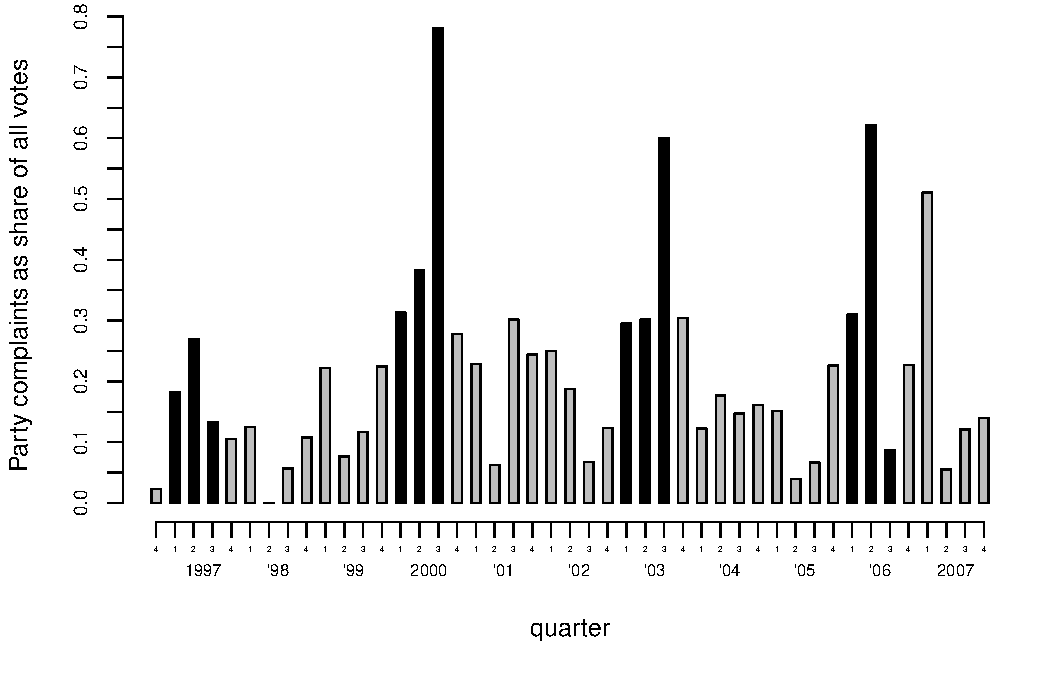
\includegraphics[width=.65\textwidth]{../../plots/lo-q-estuvo-compartido-c-memo/sharePtyComplaintsQuarter.pdf}
%  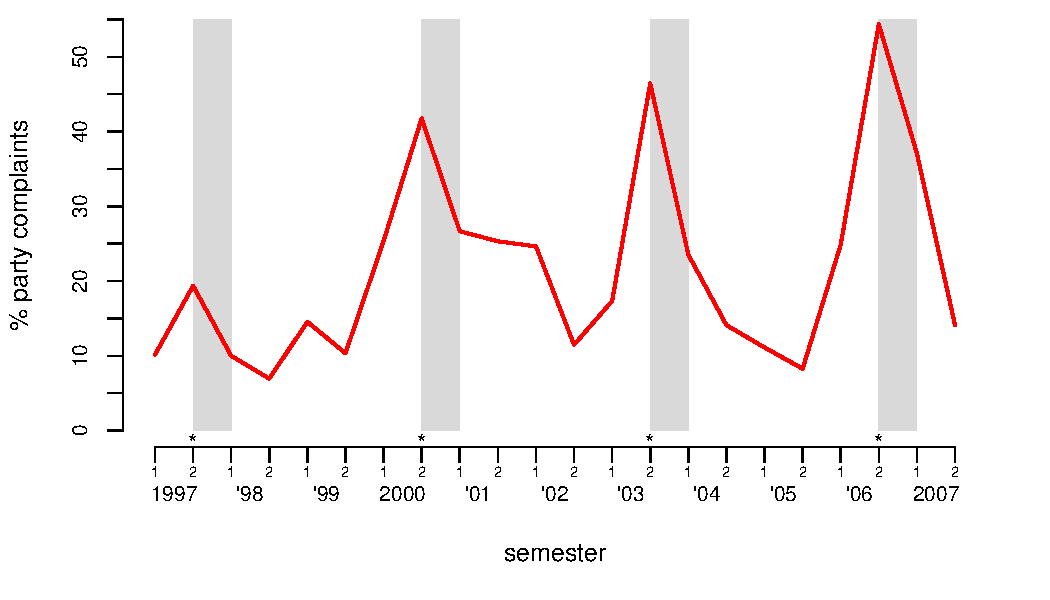
\includegraphics[width=.7\textwidth]{../../../original/graphs/ptyComplaints.pdf}
 \end{center}
\end{block}
}
%%%%%%%%%%%%%%%%%%%%%%%%%%%%%%%%%%%%%%%%%%%%%%%%%%%%%%%%%%%%%%%%%%%%%%%%%%%%%%%%%%%%%%%%%%%%%%%%
\frame {                      % SLIDE
    \frametitle{New principal and inter-semester change}
 \begin{center}
   \begin{tabular}{clcc}
    \multicolumn{2}{c}{Posterior $|x_{j,t+1}-x_{j,t}|$}&  Mean & sd \\ \hline
    a& New Congress semesters & \alert{.140}  &   .115    \\
    b& Rest                   & \alert{.108}  &   .084    \\
    c& Prob.\ a>b             & \multicolumn{2}{c}{.560} \\ \hline
   \end{tabular}
 \end{center}
}
%%%%%%%%%%%%%%%%%%%%%%%%%%%%%%%%%%%%%%%%%%%%%%%%%%%%%%%%%%%%%%%%%%%%%%%%%%%%%%%%%%%%%%%%%%%%%%%%
\frame {                      % SLIDE
    \frametitle{Gatekeeping and signal-to-noise ratio}
% \begin{center}

   \begin{tabular}{clcc}
    \multicolumn{2}{c}{Posterior $|\texttt{signal}_i|$} &  Mean & sd \\ \hline
    d& Electoral semesters    & \alert<1>{2.802} & 1.652  \\
    e& Rest                   & \alert<1>{2.484} & 1.628  \\
    f& Prob.\ d>e             & \multicolumn{2}{c}{.565} \\ \hline
   \end{tabular}

\bigskip \pause

   \begin{tabular}{clcc}
    \multicolumn{4}{c}{Posterior  $|\texttt{signal}_i|$ with ci off zero} \\
    g& Electoral semesters & \multicolumn{2}{c}{\alert<2>{64\%}} \\
    h& Rest                & \multicolumn{2}{c}{\alert<2>{46\%}} \\ \hline
%    \multicolumn{4}{c}{Abstention rates}   \\
%    i& PAN electoral semester & 0.039 & 0.054  \\
%    j& PAN rest               & 0.046 & 0.067  \\
%    k& PRI electoral semester & 0.016 & 0.021  \\
%    l& PRI rest               & 0.024 & 0.012  \\
%    m& PRD electoral semester & 0.072 & 0.031  \\
%    n& PRD rest               & 0.153 & 0.050  \\ \hline
   \end{tabular}
% \end{center}
}
%%%%%%%%%%%%%%%%%%%%%%%%%%%%%%%%%%%%%%%%%%%%%%%%%%%%%%%%%%%%%%%%%%%%%%%%%%%%%%%%%%%%%%%%%%%%%%%%
\frame {                      % SLIDE
    \frametitle{More possible tests}
    \begin{block}{Contingent median polarization}
    \begin{center}
   \begin{tabular}{lccc}
                  & \multicolumn{3}{c}{mean difference} \\
                  & election  & & rest      \\ \hline
                  & \multicolumn{3}{c}{Periods I and II}  \\
   PRI-PAN &  0.155    & >           &   0.091      \\
   PRI-PRD &  0.417    & $\approx$   &   0.413      \\
   PAN-PRD &  0.262    & $\approx$   &   0.323      \\
                  & \multicolumn{3}{c}{Period III}  \\
   PRI-PAN &  0.639    & >           &   0.369      \\
  \end{tabular}
\end{center}
\end{block}
Within-contingent cohesion
}
%%%%%%%%%%%%%%%%%%%%%%%%%%%%%%%%%%%%%%%%%%%%%%%%%%%%%%%%%%%%%%%%%%%%%%%%%%%%%%%%%%%%%%%%%%%%%%%%
\frame {                      % SLIDE
  \frametitle{Puzzles}
  \begin{enumerate}
  \item How do 3 instead of 2 parties affect delegation?
    \begin{itemize}
    \item<2-> Party quotas $\rightarrow$ power-sharing
    \item<2-> Collective principal appoints a collective agent ($\approx$ McNollgast)
    \item<2-> Same in other `autonomous' regulatory boards\\ (telecomm, energy, education...)
    \end{itemize}
  \item Unstable environment
    \begin{itemize}
    \item<3-> Principal out of business?
    \item<3-> Auto-pilot analogy still flies?
    \end{itemize}
  \item Age structure
    \begin{itemize}
    \item<4-> Mean at appointment 44 yrs, min 31
    \item<4-> Young democracies?
    \end{itemize}
  \end{enumerate}
}
%%%%%%%%%%%%%%%%%%%%%%%%%%%%%%%%%%%%%%%%%%%%%%%%%%%%%%%%%%%%%%%%%%%%%%%%%%%%%%%%%%%%%%%%%%%%%%%%
\frame {                      % SLIDE
  \frametitle{Wrap-up}
\begin{enumerate}
\item Promising routes in preliminary inspection
\item Ideal points in IFE move considerably: Short-term shocks and long-term drift?
\item Movement tied to strategic considerations?
\end{enumerate}

\pause \bigskip \bigskip

\center{\textbf{Thank you!}}
}
%%%%%%%%%%%%%%%%%%%%%%%%%%%%%%%%%%%%%%%%%%%%%%%%%%%%%%%%%%%%%%%%%%%%%%%%%%%%%%%%%%%%%%%%%%%%%%%%
    %%%%%%%%%%%%%%%%%%%%%%%%%%%%%%%%%%%%%%%
    % EXTRA SLIDES REACHED VIA HYPERLINKS %
    %%%%%%%%%%%%%%%%%%%%%%%%%%%%%%%%%%%%%%%
%%%%%%%%%%%%%%%%%%%%%%%%%%%%%%%%%%%%%%%%%%%%%%%%%%%%%%%%%%%%%%%%%%%%%%%%%%%%%%%%%%%%%%%%%%%%%%%% 
\frame {                      % SLIDE
    \frametitle{Dynamics}\label{dyn-slide}
\bigskip 

Approach 1---Martin\&Quinn (2002): 

\begin{itemize}

\item For \alert{quarter} $t$: $x_{j,t} \sim \mathrm{N}( x_{j,t-1},\text{slack})$

\item \emph{Drawback}: votes vary considerably across quarters---ideal points sensitive to sheer volume of information (Desposato), so drift may be spurious 

\end{itemize}

\bigskip

Approach 2---Bonica (2010): 

\begin{itemize}

\item Allow estimates to vary over periods of very short duration: item $i \pm k$, $k=15$

\item \alert{Vote-by-vote} estimation

\item Periods mostly overlap, constraining short-term shifts 

\item IRT instead of OC

\end{itemize}

\bigskip \flushright {\color{black!25} Back \hyperlink{analogy}{\ExternalLink}}
}
%%%%%%%%%%%%%%%%%%%%%%%%%%%%%%%%%%%%%%%%%%%%%%%%%%%%%%%%%%%%%%%%%%%%%%%%%%%%%%%%%%%%%%%%%%%%%%%%
\frame {
  \frametitle{Identification}\label{identification}
\begin{center}
 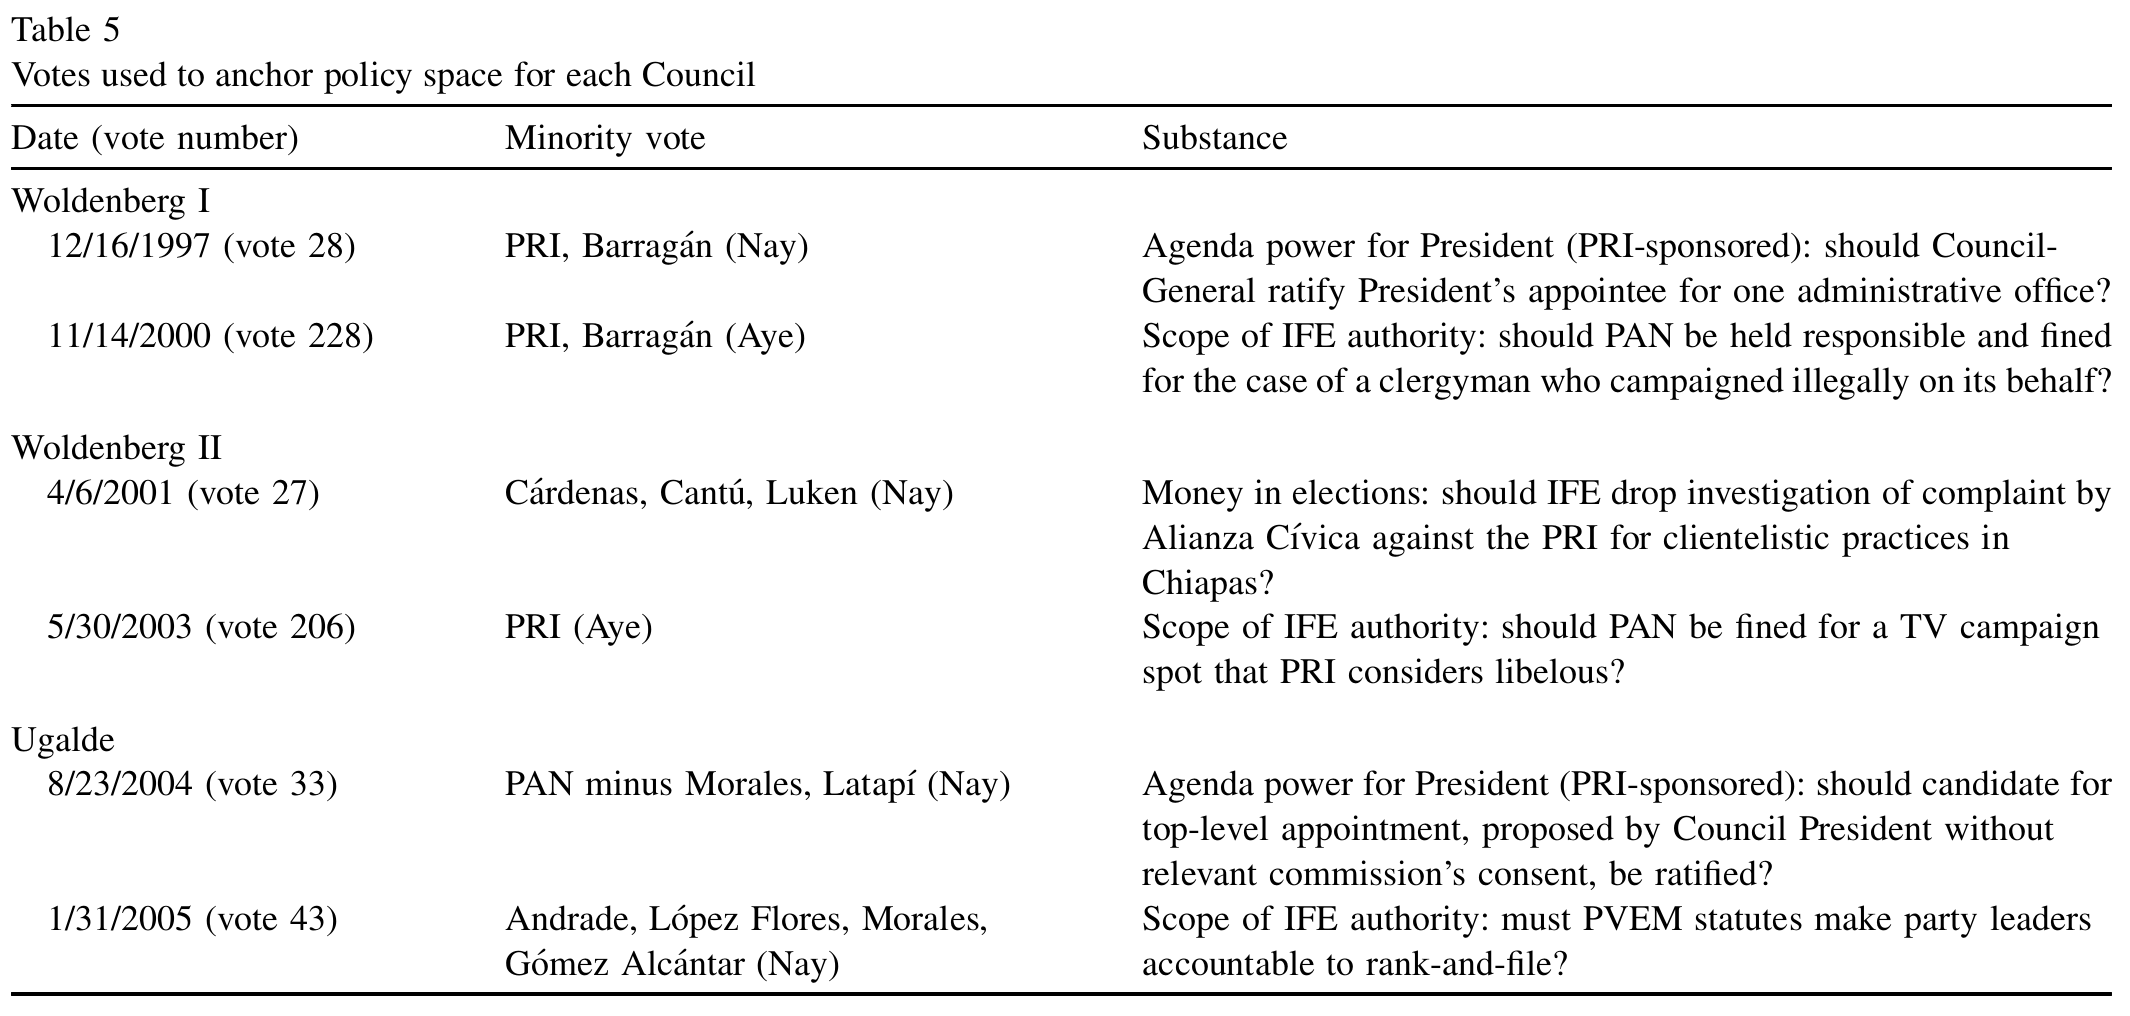
\includegraphics[width=\textwidth]{../../pics/anchor-votes.png} \\
\end{center}
\bigskip \flushright {\color{black!25} Back \hyperlink{analogy}{\ExternalLink}}
}
%%%%%%%%%%%%%%%%%%%%%%%%%%%%%%%%%%%%%%%%%%%%%%%%%%%%%%%%%%%%%%%%%%%%%%%%%%%%%%%%%%%%%%%%%%%%%%%%
\frame {                      % SLIDE
    \frametitle{Data = contested votes (in black)}\label{data}

\begin{center}

Votes: 5,202 unanimous, 1,640 contested (24\%)

\bigskip

% \includegraphics[width=\textwidth]{c:/data/rollcall/ife_cg/graphs/all+divVotsSemestre.pdf}
 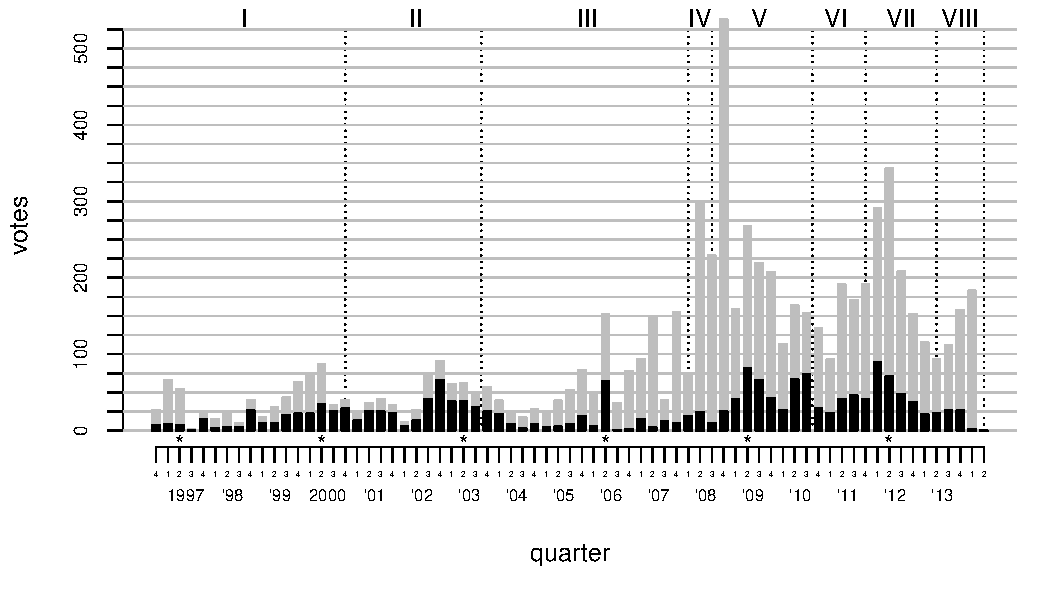
\includegraphics[width=\textwidth]{../../plots/all+divVotsQuarter.pdf}

%Presidents: Woldenberg (I--II); Ugalde (III); Vald\'es (IV--VII)
Same members within each period (I, II, ...) 

\end{center}
\flushright {\color{black!25} Back \hyperlink{analogy}{\ExternalLink}}
}
%%%%%%%%%%%%%%%%%%%%%%%%%%%%%%%%%%%%%%%%%%%%%%%%%%%%%%%%%%%%%%%%%%%%%%%%%%%%%%%%%%%%%%%%%%%%%%%%
\end{document}
%%%%%%%%%%%%%%%%%%%%%%%%%%%%%%%%%%%%%%%%%%%%%%%%%%%%%%%%%%%%%%%%%%%%%%%%%%%%%%%%%%%%%%%%%%%%%%%%


%%%%%%%%%%%%%%%%%%%%%%%%%%%%%%%%%%%%%%%%%%%%%%%%%%%%%%%%%%%%%%%%%%%%%%%%%%%%%%%%%%%%%%%%%%%%%%%% 
\frame {                      % SLIDE

    \frametitle{Mitigating agency costs (Kiewiet \& McCubbins)}

\begin{enumerate}
    \item Formal rules to appoint councilors.
    \item Informal rules (vetoes, quotas).
    \item Party signaling in committees and Council.
    \item Appeals to election tribunal (TRIFE).
    \item Impeachment threats, election reform (nuclear option).
    \item Party capture of former councilors.
\end{enumerate}

}
% %%%%%%%%%%%%%%%%%%%%%%%%%%%%%%%%%%%%%%%%%%%%%%%%%%%%%%%%%%%%%%%%%%%%%%%%%%%%%%%%%%%%%%%%%%%%%%%%

% \frame {                      % SLIDE

%     \frametitle{Food for thought}

% \begin{enumerate}

% \item<1-> Ideal points in IFE move as much as in Supreme Court.

% \item<2-> Movement seems tied to strategic
% considerations \\ (change in principal; less agenda power).

% \item<3-> Insincere voting is a problem to infer ideology. \\
% Not a problem if ideal points taken literally (voting record).

% \item<4-> Plan is to model/estimate strategic considerations.

% \item<5-> Peress 2009 on small chamber estimators.

% \end{enumerate}

% \pause \pause \pause \pause \pause

% \center{\textbf{Thank you!}}

% }

